\documentclass[11pt,twoside]{article}

\usepackage{amssymb}
\usepackage{amsmath}
\usepackage{latexsym}
\usepackage{color}
\usepackage{graphics}
\usepackage{xspace}
\usepackage{pdfpages}


% Commands for special characters
\newcommand{\mybackslash}{\char'134}
\newcommand{\myleftbracket}{\char'173}
\newcommand{\myrightbracket}{\char'175}
\newcommand{\mypercent}{\char'045}
\newcommand{\myunderscore}{\char'137}

% The 'ifthen' package supports Boolean flags
\usepackage{ifthen}
% The 'solutions' flag determines whether this is the original handout
%    or a solution
\newboolean{solutions}
\setboolean{solutions}{False}  % Default is original handout

% Uncomment the next line before starting on the solutions
\setboolean{solutions}{True}

\newcommand{\coursenumber}{CS 4124}
\newcommand{\coursetitle}{Theory of Computation}
\newcommand{\docdate}{March 25, 2024}
\newcommand{\duedate}{April 12, 2024}
\newcommand{\homeworknumber}{5}

% The document title depends on whether these are solutions
\ifthenelse{\boolean{solutions}}{% Then
\newcommand{\doctitle}{Solutions to Homework Assignment \homeworknumber}
}{% Else
\newcommand{\doctitle}{Homework Assignment \homeworknumber}
}

% The document date depends on whether these are solutions
\ifthenelse{\boolean{solutions}}{% Then
\renewcommand{\docdate}{\duedate}
}{% Else
}

% If you are the author, so put your name here
\renewcommand{\author}{Collin McDevitt}

\pagestyle{myheadings}
\markboth{\hfill\doctitle\hfill\docdate}{\docdate\hfill\doctitle\hfill}

\addtolength{\textwidth}{1.00in}
\addtolength{\textheight}{1.00in}
\addtolength{\evensidemargin}{-1.00in}
\addtolength{\oddsidemargin}{-0.00in}
\addtolength{\topmargin}{-.50in}
\setlength{\footskip}{0pt}

\newcommand{\polyreduce}{\leq_{\mathrm{P}}}

\newcounter{problem}
\setcounter{problem}{0}
\newcommand{\problem}[1]{%
\refstepcounter{problem}\noindent\textbf{[#1] \arabic{problem}.}}

\newcommand{\solution}{\bigskip\hrule\bigskip}
\newcommand{\problembreak}{\bigskip\hrule\bigskip}

\renewcommand{\theenumi}{\textbf{\Alph{enumi}}}
\renewcommand{\theenumii}{\textbf{\roman{enumii}}}

\newcommand{\emptysequence}{\Lambda}
\newcommand{\emptystring}{\varepsilon}

% Pseudocode comment symbol
\newcommand{\comment}{\textbf{//}\ \ }

% Pseudocode line numbering
\newcounter{pseudocode}
\newcommand{\firstline}{\setcounter{pseudocode}{0}\linenumber}
\newcommand{\linenumber}{\refstepcounter{pseudocode}\thepseudocode}
\newcommand{\pseudoindent}{\hspace*{26pt}}

\newcommand{\nil}{\mbox{\textsc{nil}}}

% Mathematical symbols
\newcommand{\grid}{\mathcal{G}}  % Grid graph
\newcommand{\integers}{\mathbb{Z}}  % Integers
\newcommand{\Zplus}{\mathbb{Z}^+}  % Positive integers
\newcommand{\naturals}{\mathbb{N}}  % Natural numbers
\newcommand{\reals}{\mathbb{R}}  % Real numbers

% Probability
\newcommand{\expect}[1]{\mathbf{E}\left[#1\right]}
\newcommand{\prob}[1]{\mathrm{Pr}\left[#1\right]}
\newcommand{\var}[1]{\mathrm{Var}\left[#1\right]}

% Logic
\newcommand{\NOT}[1]{\neg #1}
\newcommand{\AND}{\wedge}
\newcommand{\OR}{\vee}
\newcommand{\clause}[1]{\left(#1\right)}

\newlength{\problemoffset}
\setlength{\problemoffset}{0.5in}

% Decision problem macro
% A command for formatting decision problems a la Garey and Johnson
\newcommand{\decision}[3]{%     \decision{NAME}{INSTANCE}{QUESTION}
\begin{list}{}{
\setlength{\leftmargin}{\problemoffset}
\setlength{\rightmargin}{\problemoffset}
\setlength{\parsep}{0pt}
\setlength{\itemsep}{2pt}
\setlength{\topsep}{\itemsep}
\setlength{\partopsep}{\itemsep}
}
\item
{\textsc{#1}}
\item
{INSTANCE: #2}
\item
{QUESTION: #3}
\end{list}
}

% Optimization problem macro
\newcommand{\optimization}[3]{%  \optimization{NAME}{INSTANCE}{SOLUTION}
\begin{list}{}{
\setlength{\leftmargin}{\problemoffset}
\setlength{\rightmargin}{\problemoffset}
\setlength{\parsep}{0pt}
\setlength{\itemsep}{2pt}
\setlength{\topsep}{\itemsep}
\setlength{\partopsep}{\itemsep}
}
\item
{\rule{0pt}{14pt}\textsc{#1}}
\item
{INSTANCE: #2}
\item
{SOLUTION: #3}
\end{list}
}

\newcommand{\reaches}{\leadsto}

% Table layout
\newcommand{\toprule}{\rule[11pt]{0pt}{2pt}}
\newcommand{\bottomrule}{\rule[-6pt]{0pt}{0pt}}
\newenvironment{raggedpars}[1][2.0in]{%
\begin{minipage}[t]{#1}\raggedright\toprule}%
{\bottomrule\end{minipage}}

% Dynamic programming macros
\newlength{\arrowwidth}
\setbox3=\hbox{$\nwarrow$}
\setlength{\arrowwidth}{\wd3}
\newcommand{\optnwarrow}[1]{\if1#1\nwarrow%
\else\rule{\arrowwidth}{0pt}\fi}
\newcommand{\optuparrow}[1]{\if1#1\uparrow%
\else\rule{\arrowwidth}{0pt}\fi}
\newcommand{\optleftarrow}[1]{\if1#1\leftarrow%
\else\rule{\arrowwidth}{0pt}\fi}
% Use \tablebox to specify any combination of arrows, plus the value
\newcommand{\tablebox}[4]{%
\setlength{\arraycolsep}{0.0pt}%
\begin{array}{cc}%
\optnwarrow{#1} & \optuparrow{#2} \\%
\optleftarrow{#3} & #4%
\end{array}%
}
% Use \tableboxred to specify any combination of arrows, plus the value
% The value will be red; arrows are made red if 2 used instead of 1
\newcommand{\optnwarrowred}[1]{\if1#1\nwarrow%
\else\if2#1\textcolor{red}{\nwarrow}\else\rule{\arrowwidth}{0pt}\fi\fi}
\newcommand{\optuparrowred}[1]{\if1#1\uparrow%
\else\if2#1\textcolor{red}{\uparrow}\else\rule{\arrowwidth}{0pt}\fi\fi}
\newcommand{\optleftarrowred}[1]{\if1#1\leftarrow%
\else\if2#1\textcolor{red}{\leftarrow}\else\rule{\arrowwidth}{0pt}\fi\fi}
\newcommand{\tableboxred}[4]{%
\setlength{\arraycolsep}{0.0pt}%
\begin{array}{cc}%
\optnwarrowred{#1} &%
\optuparrowred{#2} \\%
\optleftarrowred{#3} &%
\textcolor{red}{#4}%
\end{array}%
}

% Allow really sloppy paragraphs that do not generate overfull or
%    underfull hbox's
\newenvironment{SLOPPY}{\begin{sloppypar}\hbadness=10000}{\end{sloppypar}}

% Definitions for this homework
\newcommand{\extent}[1]{\mathrm{extent}(#1)}
\newcommand{\opt}[2]{\mbox{\textsc{opt}}(#1,#2)}
\newcommand{\gap}{\mbox{\texttt{-}}}
\newcommand{\rewriterule}[2]{#1\to #2}
\newcommand{\rewrites}[2][]{\mathop{\Longrightarrow}\limits_{#1}^{#2}}
\newcommand{\reduces}{\leq}
\newcommand{\polyreduces}{\leq_P}
\newcommand{\mathsc}[1]{\mbox{\normalfont\textsc{#1}}}
\newcommand{\NP}{\mathcal{NP}}
\renewcommand{\P}{\mathcal{P}}
\newcommand{\describes}{\vdash}
\newcommand{\powerset}[1]{\mathcal{P}(#1)}

% OTM related definitions
\newcommand{\Qpollacc}{Q^{\left(\mathrm{poll,acc}\right)}}
\newcommand{\Qpollrej}{Q^{\left(\mathrm{poll,rej}\right)}}
\newcommand{\Qaut}{Q^{\left(\mathrm{aut}\right)}}
\newcommand{\blank}{\ensuremath\fbox{\sc b}}

\begin{document}

\thispagestyle{empty}

\begin{center}
\begin{tabular}{lcr}
\multicolumn{3}{c}{\Large\textbf{\coursenumber}}
\\[0.04in]
\multicolumn{3}{c}{\Large\textbf{\doctitle}}
% If these are solutions, then include the author's (student's) name
\ifthenelse{\boolean{solutions}}{% Then
\\[0.04in]\multicolumn{3}{c}{\large\textbf{\author}}
}{} % Else omit
% If these are solutions, then the date is the due date
\ifthenelse{\boolean{solutions}}{% Then
\\[0.10in]\multicolumn{3}{c}{\duedate}
}{% Else, put given and due dates
\\[0.10in]
\textbf{Given:} \docdate
& \hspace*{1.0in} &
\textbf{Due:} \duedate
}
\end{tabular}
\end{center}

% If these are solutions, then we do not include the directions
\ifthenelse{\boolean{solutions}}{} % No directions
{
% Original document includes directions
\begingroup % This allows an argument that contains multiple paragraphs
\paragraph{General directions.}
The point value of each problem is shown in [ ].
Each solution must include all details and
an explanation of why the given solution is correct.
\textbf{\textcolor{red}{In particular,
write complete sentences.
A correct answer without an explanation is worth no credit.}}
The completed assignment must be submitted on Canvas as a PDF by 5:00 PM
on \duedate.
\textbf{No late homework will be accepted.}

\paragraph{Digital preparation of your solutions is mandatory.
This includes digital preparation of any drawings; see syllabus
concerning neat drawings included in \LaTeX\ solutions.}
\textbf{Use of \LaTeX\ is required.
Also,
please include your name.}

\paragraph{Use of \LaTeX\ (required).}
\begin{itemize}
\item Retrieve this \LaTeX\ source file,
named
\texttt{homework\homeworknumber.tex},
from the course web site.
\item Rename the file
\textit{$<$Your VT PID$>$}\texttt{{\myunderscore}solvehw\homeworknumber.tex},
For example,
for the instructor,
the file name would be
\texttt{heath{\myunderscore}solvehw\homeworknumber.tex}.

\item
Use a \textbf{text editor}
(such as \texttt{vi}, \texttt{emacs}, or \texttt{pico})
to accomplish the next three steps.
Alternately,
use Overleaf as your \LaTeX\ platform.

\item
Uncomment the line

\texttt{{\mypercent} 
{\mybackslash}setboolean{\myleftbracket}solutions{\myrightbracket}%
{\myleftbracket}True{\myrightbracket}}

in the document preamble by deleting the \texttt{\mypercent}.

\item
Find the line

\texttt{{\mybackslash}renewcommand%
{\myleftbracket}{\mybackslash}author{\myrightbracket}%
{\myleftbracket}Lenwood S. Heath{\myrightbracket}}

and replace the instructor's name with your name.

\item
Enter your solutions where you find
the \LaTeX\ comments

\texttt{{\mypercent} PUT YOUR SOLUTION HERE}

\item
Generate a PDF and turn it in on Canvas by 5:00 PM on \duedate.
\end{itemize}
\endgroup

\problembreak

\newpage

}

\problem{50}
Let
$\mathcal{R}_1$
be the (simplified) regular expression $(ba)^\star + (abb)(abb)^\star$.

{\bfseries
Construct an $\emptystring$-NFA $N_1$
that accepts the language denoted by $\mathcal{R}_1$.
You should employ the construction
given in class or in the textbook for inspiration,
but you do not have to follow the construction precisely.
Use reason to construct your $N_1$
and justify your reasoning.
Give $N_1$ as a labeled directed graph or state diagram.
Please draw it neatly!
}

\solution

This was constructed by first creating two $\emptystring-$NFA the first one located at the top recognizes $(ba)^\star$ this is seen as it accepts the empty string and if it does receive a string in order for it to accept it must take the path $q_1\longrightarrow q_2 \longrightarrow q_3 \longrightarrow q_1$ which can only be traversed by the string $ba\emptystring$. The epsilon ensures that $(ba)^\star$ will be recognized.

The second $\emptystring-$NFA is located at the bottom and recognizes $(abb)(abb)^\star$ this is seen as it first must traverse $q_4\longrightarrow q_5 \longrightarrow q_6 \longrightarrow q_7$ to reach an accepting state. This can only be done by the string $abb$ after it is in state $q_7$ there is an epsilon transition back to $q_4$ which ensures that $(abb)(abb)^\star$ will also be recognized. Both these $\emptystring-$NFA are combined with the initial state $q_0$ and a $\emptystring$ transition to their initial states.


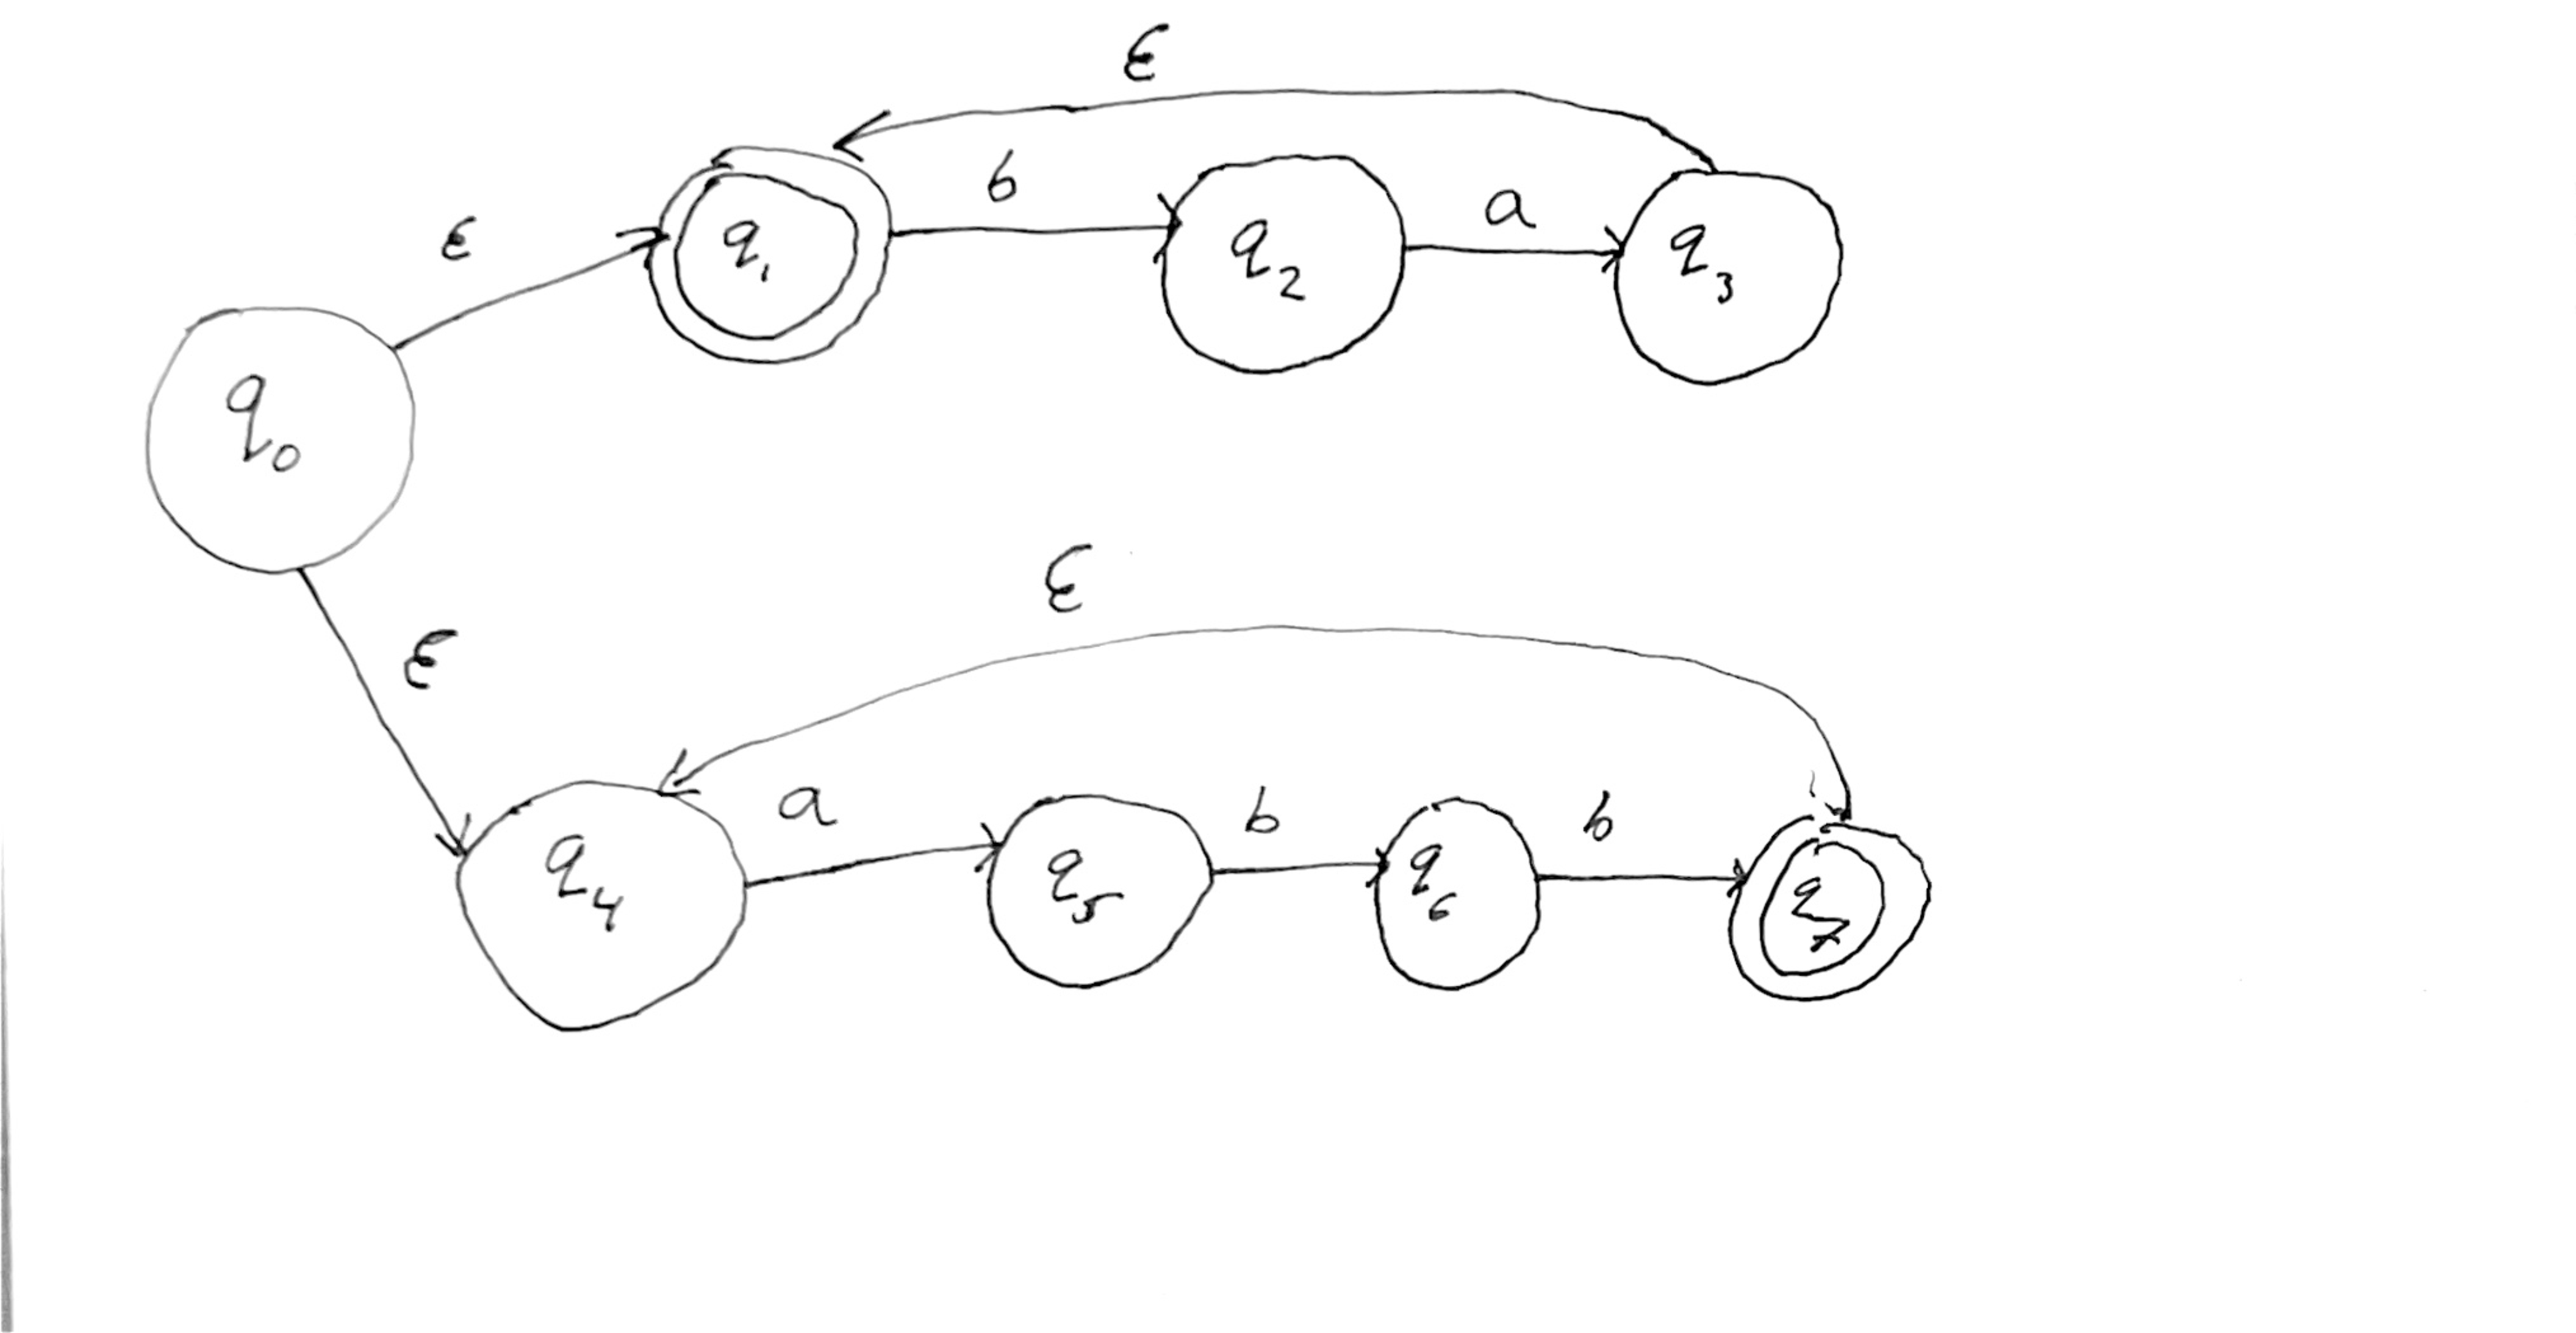
\includepdf[pages=-]{2st.pdf}


% PUT YOUR SOLUTION HERE

\problembreak

\problem{50}
Let
$N_2$
be the $\emptystring$-NFA in Figure~\ref{figure:e-NFA_Problem2}.

{\bfseries
\begin{enumerate}
\item
Compute the $\emptystring$-reachability set $E(q)$ of each state $q$ of $N_2$.
{
    \begin{align*}
        E(q_0)&=\{q_0,q_1,q_2\}\\
        E(q_1)&=\{q_1\}\\
        E(q_2)&=\{q_2\}
    \end{align*}


}

\item

\begin{displaymath}
\begin{array}{|c|l|}
\hline
bb
&
q_0 \stackrel{b}{\longrightarrow} q_1\stackrel{b}{\longrightarrow} q_2 
\\\hline cb & q_0 \stackrel{\emptystring}{\longrightarrow} q_1 \stackrel{c}{\longrightarrow} q_1 \stackrel{b}{\longrightarrow}q_2 \\ \hline \emptystring & q_0 \stackrel{\emptystring}{\longrightarrow} q_2 \\ \hline 
c & q_0 \stackrel{c}{\longrightarrow } q_2 \\ \hline 
b & q_0 \stackrel{\emptystring}{\longrightarrow} q_1 \stackrel{b}{\longrightarrow} q_2 \\ \hline
ab & q_0 \stackrel{\emptystring}{\longrightarrow} q_1 \stackrel{a}{\longrightarrow} q_0 \stackrel{\emptystring}{\longrightarrow}q_1 \stackrel{b}{\longrightarrow}q_2 \\ \hline
cc & q_0 \stackrel{\emptystring}{\longrightarrow} q_1 \stackrel{c}{\longrightarrow} q_0 \stackrel{c}{\longrightarrow} q_2 \\ \hline
ac & q_0 \stackrel{\emptystring}{\longrightarrow} q_1 \stackrel{a}{\longrightarrow} q_0 \stackrel{c}{\longrightarrow} q_2 \\ \hline

ca & q_0 \stackrel{\emptystring}{\longrightarrow} q_1 \stackrel{c}{\longrightarrow} q_1 \stackrel{a}{\longrightarrow} q_0 \stackrel{\emptystring}{\longrightarrow} q_2 \\ \hline
ba & q_0 \stackrel{b}{\longrightarrow} q_1 \stackrel{a}{\longrightarrow} q_0 \stackrel{\emptystring}{\longrightarrow} q_2 \\ \hline
a & q_0 \stackrel{\emptystring}{\longrightarrow}q_1 \stackrel{a}{\longrightarrow} q_0 \stackrel{\emptystring}{\longrightarrow}q_2 \\ \hline

\end{array}
\end{displaymath}
\item
Use the power set construction
to obtain a DFA $M_2$ equivalent to $N_2$.
Give $M_2$ as a labeled directed graph or state diagram.
Please draw it neatly!
\end{enumerate}
}

\solution


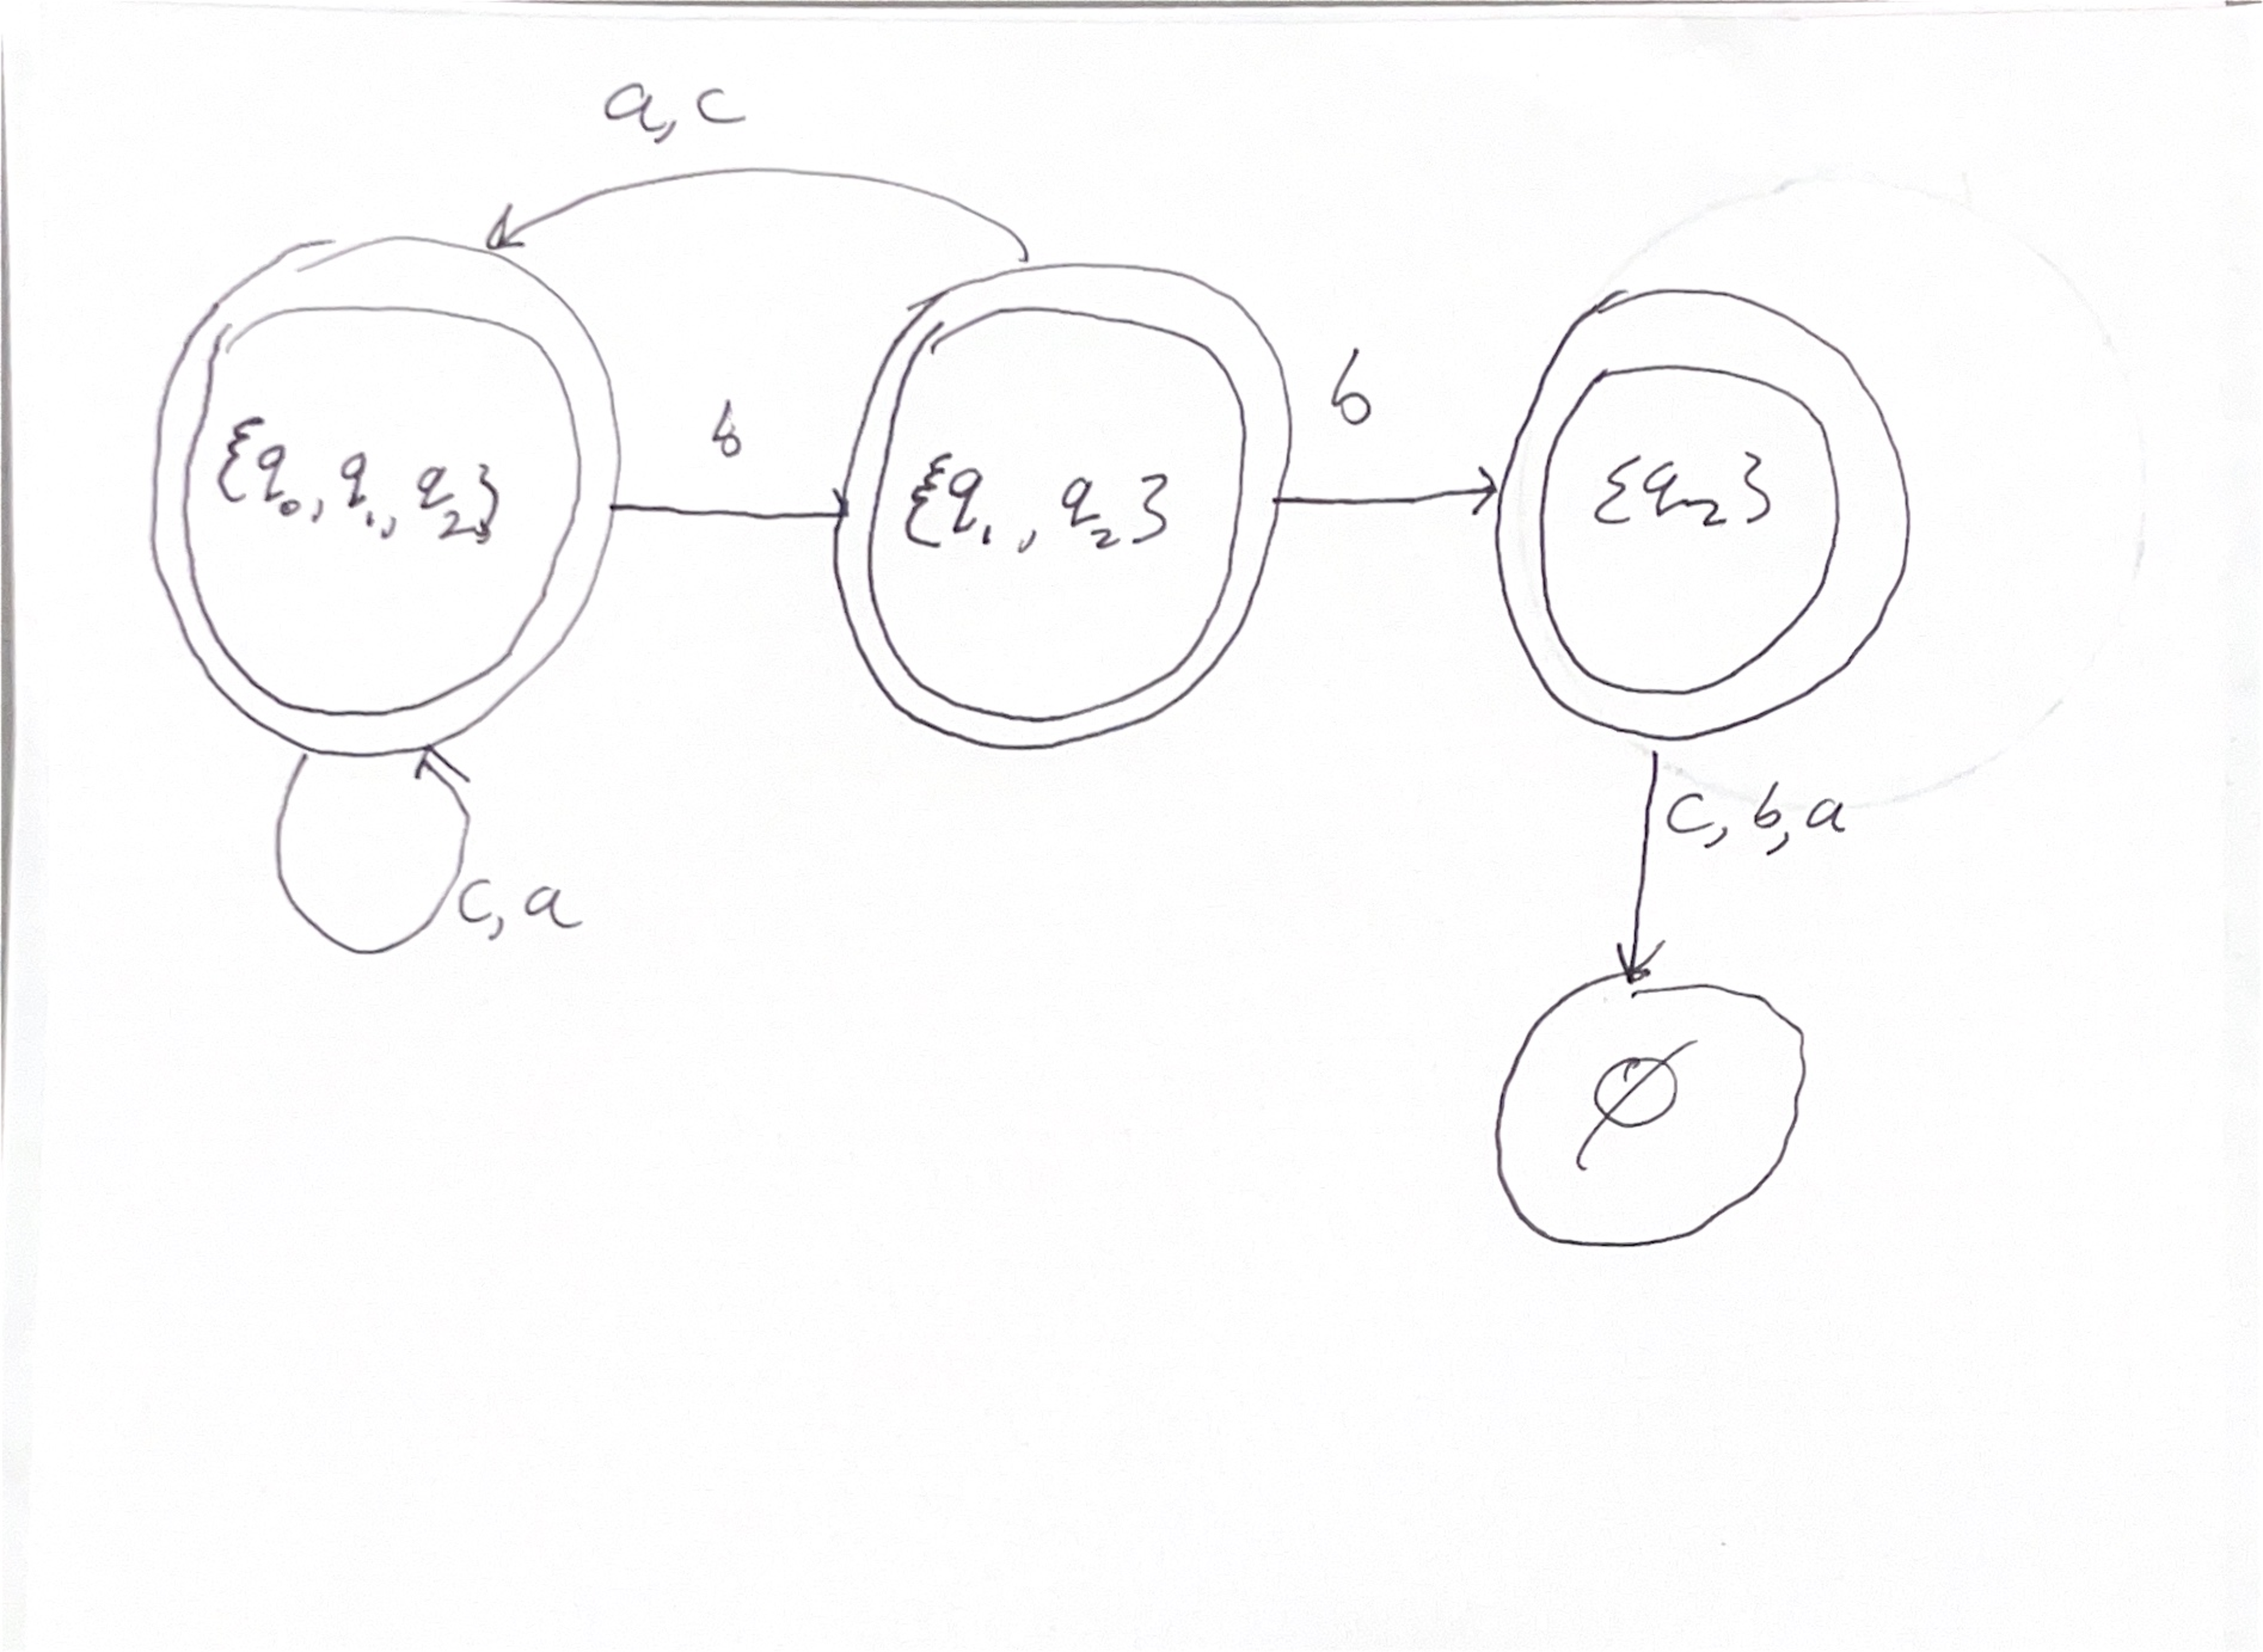
\includepdf[pages=-]{3rd.pdf}


\end{document}
